\documentclass[12pt]{article}
\PassOptionsToPackage{hidelinks}{hyperref} 
\usepackage{amsmath}
\usepackage{tikz}
\usepackage{geometry}
\usepackage{bookmark}
\usepackage{graphicx}
\usetikzlibrary{decorations.pathreplacing}

\geometry{margin=2.5cm}

\title{N-Body simulation in OpenCl with a AMD iGPU}
\author{}
\date{}

\begin{document}

\begin{titlepage}
    \centering

    \vspace*{2cm}

    {\Huge \textbf{N-Body Simulation}}\\[0.4cm]
    {\Large Using OpenCL on an AMD iGPU}

    \vspace{2cm}

    {\Large \textbf{Nagy Levente}}

    \vspace{1cm}

    {\large \today}

    \vfill

    \rule{\textwidth}{0.4pt}

    \vspace{0.3cm}

    {\large
    Eötvös Lóránd University
    }

\end{titlepage}

\pagebreak

\tableofcontents


\pagebreak

\section{Introduction}

\subsection{N-Body simulation}

An N-body simulation models the motion of \textbf{N} particles in space,
where each particle is influenced by physical forces such as gravity,
defined by the gravitational constant \textbf{G}.

\section{Problem}
\subsection{General N-Body problem}

The general N-body problem has no closed-form analytical solution for N >= 3 (the famous three-body problem).

\subsection{N-Body computing}
Computing the forces from each body acting on every other body is costly when \textbf{N} is a big number.
A simple brute force algorithm time complexity is \[O(n^2)\]
For a better algorithm there exists the Barnes-Hut algorithm which time complexity is \[O(n \log(n))\]
So its a much better solution for computing the forces. We can plot them to see the difference

\subsection{Barnes-Hut alogithm}
\subsubsection{Idea}
The Barnes-Hut algorithm divides the space where the bodies located into 8 smaller chunks
if there is more than 1 body is in a chunk. After recursively doing this for every body
we are left with an Octree (each parent can have up to 8 children).
In the given tree each node represtens a 3Dimensional space with a body.
Than we compute the \textbf{COM} (Center Of Mass) of each node and use this formula
\[\frac{s}{d} < \theta  \] 
where:
\begin{itemize}
    \item $s$ is the size of the region
    \item $d$ is the distance to the center of mass
    \item $\theta$ controls the trade-off between accuracy and performance
\end{itemize}
To determine if 2 nodes of the tree can be used as 1, reducing the computeitation steps we have to do, reducing the time complexity
to just \[O(n \log(n))\]

\begin{center}
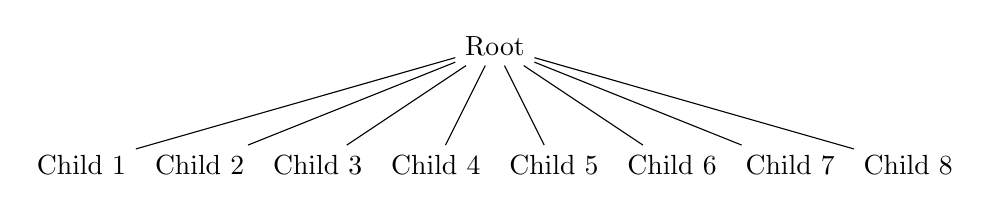
\begin{tikzpicture}
\node {Root}
child {node {Child 1}}
child {node {Child 2}}
child {node {Child 3}}
child {node {Child 4}}
child {node {Child 5}}
child {node {Child 6}}
child {node {Child 7}}
child {node {Child 8}};
\end{tikzpicture}
\end{center}

\subsubsection{Problem with the algorithm on GPU}
The Barnes-Hut algorithm relies on tree traversal, which is naturally recursive.
However, recursion is inefficient or unsupported in GPU programming models such as OpenCL.
Therefore, the algorithm must be reformulated using iterative techniques
and explicit memory structures to work.

\section{Solution}
This section is going to describe the solution and the implementation of the Barnes-Hut alogithm on the GPU
\subsection{Steps}
\begin{enumerate}
    \item Computing the bounding box containing all of the bodies
    \item Build the octree and instert the bodies into it
    \item Summerize the information of the bodies (Center Of Mass)
    \item Sorting the bodies based on spatial distance (not necessary but helps with the performance)
    \item Calculating the force
    \item Applying the force to each body, updating position and velocities
    \item Passing the global data to the pipline
\end{enumerate}

\subsection{Data Structure}

Efficient data representation is critical for achieving high performance on the GPU.
Instead of using a traditional pointer-based tree structure, the simulation uses a
\textbf{linearized octree} stored in contiguous memory buffers.

\paragraph{Overview}

All simulation data is stored in flat arrays in global memory.
Each index represents either a body or an internal node of the octree.

\begin{itemize}
    \item The first $N$ entries correspond to physical bodies (leaf nodes)
    \item The remaining entries represent internal octree nodes (parents and root)
\end{itemize}
The size of the array is chosen to be approximately $2N$, which provides a safe upper bound.
In an octree, each body corresponds to at most one leaf node, and the number of internal nodes
is strictly less than the number of bodies. Therefore, the total number of nodes
(bodies plus internal nodes) never exceeds $2N$.  


\begin{center}

    
    Array
    
    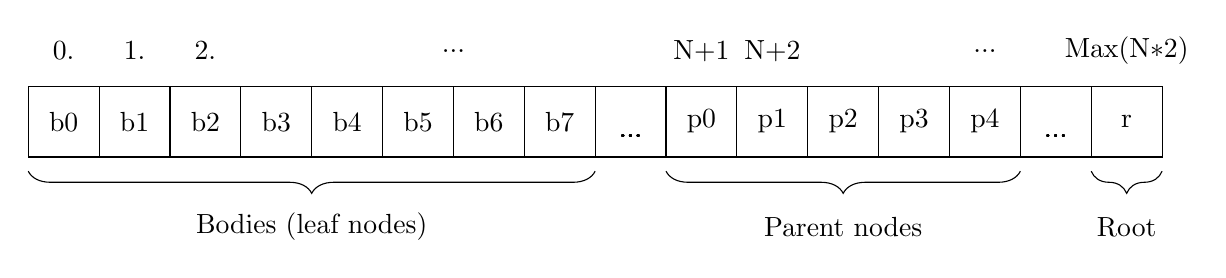
\begin{tikzpicture}[scale=0.9]

    \node at (0.5, 3.5) {0.};
    \node at (1.5, 3.5) {1.};
    \node at (2.5, 3.5) {2.};
    \node at (6.0, 3.5) {...};
    \node at (9.5, 3.5) {N+1};
    \node at (10.5, 3.5) {N+2};
    \node at (13.5, 3.5) {...};
    \node at (15.5, 3.5) {Max(N$*2$)};

    \foreach \i in {0,...,15} 
    {
        \draw (\i,2) rectangle (\i+1,3);
    }

    \foreach \i/\label in {0/b0,1/b1,2/b2,3/b3,4/b4,5/b5,6/b6,7/b7} 
    {
        \node at (\i+0.5,2.5) {\label};
        \node at (8.5,2.3) {...};
    }

    \foreach \i/\label in {9/p0,10/p1,11/p2,12/p3,13/p4} 
    {
        \node at (\i+0.5,2.5) {\label};
        \node at (14.5,2.3) {...};
    }

    \node at (15.5,2.5) {r};

    \draw[decorate,decoration={brace,mirror,amplitude=8pt}]
    (0.0,1.8) -- (8,1.8)
    node[midway,yshift=-20pt]{Bodies (leaf nodes)};

    \draw[decorate,decoration={brace,mirror,amplitude=8pt}]
    (9.0,1.8) -- (14,1.8)
    node[midway,yshift=-20pt]{Parent nodes};

    \draw[decorate,decoration={brace,mirror,amplitude=8pt}]
    (15.0,1.8) -- (16,1.8)
    node[midway,yshift=-20pt]{Root};

    \end{tikzpicture}
\end{center}

\subsection{Buffers}

\paragraph{Position and Mass Storage}

The positions and masses are stored in separate arrays:

\begin{itemize}
    \item \texttt{pos\_x, pos\_y, pos\_z} — coordinates of bodies and nodes
    \item \texttt{mass} — mass of each body or aggregated node
\end{itemize}

For internal nodes, the position represents the \textbf{center of mass (COM)}.

\paragraph{Tree Structure Representation}

The octree structure is encoded using index-based arrays:

\begin{itemize}
    \item \texttt{child} — stores indices of the 8 children for each node
    \item \texttt{start} — marks the beginning of a node's body range
\end{itemize}

Each node has exactly 8 child slots:

\[
\texttt{child[node * 8 + i]}, \quad i \in [0,7]
\]

Special values are used to indicate state:

\begin{itemize}
    \item \texttt{EMPTY (-1)} — no child present
    \item \texttt{LOCKED (-2)} — node is being modified by another thread
\end{itemize}

\paragraph{Node Properties}

Additional arrays store per-node metadata:

\begin{itemize}
    \item \texttt{nodeSize} — spatial size (half-width) of the node
    \item \texttt{nodeCount} — number of bodies contained in the node
\end{itemize}

The root node is stored at a fixed index (\texttt{NUMBER\_OF\_NODES}) and represents the bounding volume of the entire system.

\begin{itemize}
    \item \texttt{NUMBER\_OF\_NODES (numNodes)} — Size of the flat array $\rightarrow 2N$
\end{itemize}

\paragraph{Auxiliary Buffers}

Several additional buffers are used during computation:

\begin{itemize}
    \item \texttt{sorted} — stores bodies ordered by spatial distance
    \item \texttt{accX, accY, accZ} — accumulated forces
    \item \texttt{vx, vy, vz} — velocities of bodies
\end{itemize}

\paragraph{Advantages of the Approach}

This data-oriented design has several advantages:

\begin{itemize}
    \item Avoids dynamic memory allocation and recursion
    \item Enables parallel processing across threads
    \item Improves cache efficiency and memory coalescing
    \item Allows interoperability with OpenGL buffers for rendering
\end{itemize}

\paragraph{Summary}

By representing the octree as a set of flat arrays, the simulation achieves a structure
that is well-suited for GPU execution while still supporting efficient Barnes-Hut traversal.

\subsection{Kernels}

\subsubsection{Bounding Box Kernel}

The purpose of this kernel is to compute the global bounding box that contains all bodies in the simulation.
This bounding box is later used to initialize the root node of the octree structure required by the Barnes-Hut algorithm.

\paragraph{Overview}

The kernel performs a parallel reduction to determine the minimum and maximum coordinates along each axis ($x$, $y$, $z$).
Each work-group processes a subset of the bodies and computes a local bounding box, which is then combined into a global result.

\paragraph{Step 1: Local Reduction}

Each work-item iterates over the input data using a strided access pattern:

\[
i = \text{localId} + \text{groupId} \cdot \text{localSize}
\]

This ensures that all bodies are covered efficiently across all work-groups.

For each assigned body, the thread updates its local minimum and maximum values:
\begin{itemize}
    \item $x_{\min}, x_{\max}$
    \item $y_{\min}, y_{\max}$
    \item $z_{\min}, z_{\max}$
\end{itemize}

These values are stored in shared local memory to allow fast intra-group communication.

\paragraph{Step 2: Parallel Reduction in Local Memory}

A tree-based reduction is performed within each work-group:

\begin{itemize}
    \item At each step, half of the threads combine their values with a partner thread
    \item This continues until thread $0$ holds the result for the entire work-group
\end{itemize}

This reduces the per-group bounding box to a single set of values.

\paragraph{Step 3: Global Reduction}

The first thread of each work-group writes its result into global memory.
An atomic counter (\texttt{blockCount}) is used to detect when all work-groups have finished.
The last work-group to finish performs a final reduction over all partial results to compute the global bounding box.

\paragraph{Step 4: Root Node Initialization}

Once the global bounding box is known, the kernel initializes the root node of the octree:

\begin{itemize}
    \item The center of the root node is computed as:
    \[
    \mathbf{c} = \frac{1}{2} (\mathbf{min} + \mathbf{max})
    \]
    
    \item The size (radius) of the node is:
    \[
    r = \frac{1}{2} \max \left(
        x_{\max} - x_{\min},
        y_{\max} - y_{\min},
        z_{\max} - z_{\min}
    \right)
    \]
\end{itemize}

The root node is stored at index \texttt{NUMBER\_OF\_NODES} and initialized with:
\begin{itemize}
    \item Position = center of the bounding box
    \item Size = computed radius
    \item Mass = $-1$ (indicating an internal node)
    \item Children = \texttt{EMPTY}
\end{itemize}

\paragraph{Synchronization}

The kernel uses:
\begin{itemize}
    \item \texttt{barrier()} for synchronization within a work-group
    \item \texttt{atomic\_inc()} to coordinate between work-groups
\end{itemize}

This ensures correct ordering despite the lack of global synchronization in OpenCL.

\paragraph{Result}

At the end of execution:
\begin{itemize}
    \item The global bounding box is computed
    \item The root node of the octree is initialized
    \item The simulation is ready for tree construction
\end{itemize}

\subsubsection{Build Tree Kernel}

The purpose of this kernel is to construct the octree by inserting each body
into the hierarchical spatial structure. This step transforms the flat list
of bodies into a tree representation that enables efficient Barnes-Hut force computation.

\paragraph{Overview}

Each work-item is responsible for inserting one or more bodies into the tree.
The insertion process starts at the root node and iteratively descends through
the tree until a suitable location for the body is found.

The kernel avoids recursion by using an iterative traversal approach,
which is required for efficient execution on the GPU.

\paragraph{Step 1: Initialization}

The root node is retrieved from the precomputed bounding box:

\begin{itemize}
    \item Position: $(x_{\text{root}}, y_{\text{root}}, z_{\text{root}})$
    \item Size: \texttt{radius}
\end{itemize}

Each thread processes bodies in a strided manner:

\[
\text{bodyIdx} += \text{localSize} \cdot \text{numGroups}
\]

This ensures all bodies are distributed evenly across threads.

\paragraph{Step 2: Tree Traversal}

For each body, the algorithm determines which of the 8 octants it belongs to.
This is encoded as a 3-bit index:

\begin{itemize}
    \item Bit 0: $x$ comparison
    \item Bit 1: $y$ comparison
    \item Bit 2: $z$ comparison
\end{itemize}

This produces a value in the range $[0,7]$, identifying the child node.

The traversal continues as long as the selected child is an internal node:
\begin{itemize}
    \item Update the current node
    \item Reduce the node size (half each level)
    \item Recompute the child index
\end{itemize}

\paragraph{Step 3: Concurrent Insertion}

When a leaf position is reached, the kernel attempts to insert the body.
Since multiple threads may access the same node, atomic operations are required.

\begin{itemize}
    \item \texttt{atom\_cmpxchg()} is used to lock the target child slot
    \item \texttt{LOCKED (-2)} indicates that another thread is modifying the node
\end{itemize}

Three cases are possible:

\begin{enumerate}
    \item \textbf{Empty slot:}  
    The body is inserted directly.

    \item \textbf{Occupied by another body:}  
    A new internal node is created, and both bodies are redistributed
    into its children.

    \item \textbf{Node already being modified:}  
    The thread retries until the slot becomes available.
\end{enumerate}

\paragraph{Step 4: Node Subdivision}

If two bodies fall into the same region, the space is subdivided:

\begin{itemize}
    \item A new node is allocated using an atomic decrement on \texttt{bottom}
    \item The node's position and size are computed based on the parent
    \item The existing body is moved into the correct child of the new node
\end{itemize}

This process repeats until the bodies are separated or a stopping condition is reached.

\paragraph{Stopping Conditions}

To prevent infinite subdivision, two limits are enforced:

\begin{itemize}
    \item Minimum cell size: \texttt{currentR < SOFTENING}
    \item Maximum depth: typically 64 levels
\end{itemize}

If either condition is met, the body is forcefully inserted without further subdivision.

\paragraph{Step 5: Depth Tracking}

Each thread tracks the maximum depth reached during insertion.
At the end of execution, a global maximum is computed using:

\begin{itemize}
    \item \texttt{atom\_max(maxDepth, localMaxD)}
\end{itemize}

This value is useful for performance analysis and debugging.

\paragraph{Synchronization}

The kernel relies on:

\begin{itemize}
    \item Atomic operations for safe concurrent updates
    \item Memory fences (\texttt{mem\_fence}) to ensure visibility of writes
\end{itemize}

No global synchronization is required, allowing the kernel to scale efficiently.

\paragraph{Result}

After execution:

\begin{itemize}
    \item All bodies are inserted into the octree
    \item Internal nodes are created where necessary
    \item The tree structure is fully constructed and ready for traversal
\end{itemize}

\subsubsection{Summarize Tree Kernel}

The purpose of this kernel is to compute aggregate information for each internal
node of the octree. In particular, it calculates the \textbf{total mass} and
\textbf{center of mass (COM)} for every node, which are essential for the
Barnes-Hut force approximation.

\paragraph{Overview}

After the tree structure has been constructed, internal nodes do not yet contain
valid physical data. This kernel traverses the tree bottom-up and computes:

\begin{itemize}
    \item The total mass of each node
    \item The center of mass position
    \item The number of bodies contained in the node
\end{itemize}

Unlike other kernels, this step is executed by a \textbf{single work-item}
(\texttt{global\_id == 0}). This simplifies synchronization and guarantees
correct ordering of computations.

\paragraph{Step 1: Iteration over Nodes}

The kernel iterates over all internal nodes:

\[
\texttt{for (node = bottom; node <= NUMBER\_OF\_NODES; node++)}
\]

\begin{itemize}
    \item \texttt{bottom} marks the first internal node
    \item \texttt{NUMBER\_OF\_NODES} corresponds to the root node
\end{itemize}

Leaf nodes (bodies) are skipped since their mass and position are already known.

\paragraph{Step 2: Accumulating Child Information}

For each internal node, all 8 child slots are examined:

\begin{itemize}
    \item If a child is \texttt{EMPTY}, it is ignored
    \item Otherwise, its contribution is accumulated
\end{itemize}

The following values are computed:

\begin{itemize}
    \item Total mass:
    \[
    M = \sum_i m_i
    \]
    
    \item Weighted position:
    \[
    \mathbf{c} = \sum_i m_i \mathbf{x}_i
    \]
    
    \item Body count:
    \[
    \text{count} =
    \begin{cases}
        1 & \text{if child is a body} \\
        \texttt{nodeCount[child]} & \text{if child is an internal node}
    \end{cases}
    \]
\end{itemize}

\paragraph{Step 3: Computing Center of Mass}

If the total mass is non-zero, the center of mass is computed as:

\[
\mathbf{x}_{\text{COM}} = \frac{\sum_i m_i \mathbf{x}_i}{\sum_i m_i}
\]

This value is written back into the node's position arrays
(\texttt{x}, \texttt{y}, \texttt{z}).

\paragraph{Step 4: Updating Node Data}

Each node is updated with:

\begin{itemize}
    \item \texttt{mass[node]} — total mass of the subtree
    \item \texttt{x[node], y[node], z[node]} — center of mass
    \item \texttt{nodeCount[node]} — number of bodies contained
\end{itemize}

A memory fence is used to ensure that writes are visible before continuing:

\begin{itemize}
    \item \texttt{mem\_fence(CLK\_GLOBAL\_MEM\_FENCE)}
\end{itemize}

\paragraph{Design Choice}

This kernel is intentionally executed sequentially on a single thread:

\begin{itemize}
    \item Ensures correct bottom-up dependency resolution
    \item Avoids complex synchronization between work-items
    \item The workload is relatively small compared to force computation
\end{itemize}

Although parallelization is possible, the overhead would outweigh the benefits
for this stage of the algorithm.

\paragraph{Result}

After execution:

\begin{itemize}
    \item All internal nodes contain valid mass and center of mass values
    \item Each node knows how many bodies it represents
    \item The octree is fully prepared for efficient Barnes-Hut force evaluation
\end{itemize}

\subsubsection{Sort Kernel}

The purpose of this kernel is to reorder bodies in memory according to their spatial locality,
as defined by the octree structure. This step is not strictly required for correctness,
but it significantly improves performance in later stages, especially during force computation,
by improving memory coherence and cache efficiency.

\paragraph{Overview}

The kernel traverses the octree and produces a linear ordering of bodies in the array
\texttt{sorted}. The ordering ensures that bodies that are close in space are also
close in memory.

This improves:
\begin{itemize}
    \item Memory coalescing on the GPU
    \item Cache utilization
    \item Traversal efficiency in the force computation step
\end{itemize}

\paragraph{Execution Model}

The kernel is executed by a single work-item:

\begin{itemize}
    \item Only the thread with \texttt{global\_id = 0} performs the computation
    \item This is sufficient since the operation is inherently sequential
\end{itemize}

\paragraph{Tree Traversal}

The traversal starts from the root node and proceeds downwards:

\begin{itemize}
    \item Nodes are processed in reverse order, from the root toward the leaves
    \item The variable \texttt{btm} marks the lowest internal node in the tree
\end{itemize}

For each node:
\begin{itemize}
    \item The starting index \texttt{s = start[cell]} determines where its data should be written
    \item If \texttt{start[cell] < 0}, the node is skipped
\end{itemize}

\paragraph{Processing Children}

Each node has up to 8 children. For each child:

\begin{itemize}
    \item \textbf{Internal node ($c \geq$ NUM\_BODIES):}
    \begin{itemize}
        \item Assign its starting index:
        \[
        \texttt{start[c] = s}
        \]
        \item Increment $s$ by the number of bodies contained in that subtree:
        \[
        s \mathrel{+}= \texttt{nodeCount[c]}
        \]
    \end{itemize}

    \item \textbf{Leaf node (body):}
    \begin{itemize}
        \item Store the body index in the sorted array:
        \[
        \texttt{sorted[s++] = c}
        \]
    \end{itemize}
\end{itemize}

\paragraph{Result}

After execution:

\begin{itemize}
    \item The array \texttt{sorted} contains all bodies in a spatially coherent order
    \item The \texttt{start} array defines contiguous ranges for each subtree
\end{itemize}

\paragraph{Benefits}

This ordering provides several advantages:

\begin{itemize}
    \item Bodies that are spatially close are processed together
    \item Memory accesses become more predictable and efficient
    \item Subsequent kernels (e.g., force computation) achieve better performance
\end{itemize}

\paragraph{Summary}

The sort kernel converts the hierarchical octree structure into a linear memory layout
that preserves spatial locality. This transformation is key for achieving high performance
on GPU architectures.

\subsubsection{Force Kernel}

The purpose of this kernel is to compute the gravitational acceleration acting on each body
using the Barnes-Hut approximation. This is the most computationally intensive part of the simulation.

\paragraph{Overview}

Each work-item is responsible for computing the net force acting on a single body.
Instead of evaluating all pairwise interactions (\(O(N^2)\)), the kernel traverses the octree
and approximates distant groups of bodies as a single mass.

This reduces the complexity to approximately \(O(N \log N)\).

\paragraph{Body Assignment}

Each thread processes one body:

\begin{itemize}
    \item The index is obtained via \texttt{get\_global\_id(0)}
    \item The actual body index is retrieved from the \texttt{sorted} array
\end{itemize}

This ensures that bodies are processed in a spatially coherent order.

\paragraph{Initialization}

For each body:

\begin{itemize}
    \item Its position \((b_x, b_y, b_z)\) is loaded
    \item Accumulated acceleration \((a_x, a_y, a_z)\) is initialized to zero
\end{itemize}

\paragraph{Tree Traversal}

The octree is traversed using an explicit stack:

\begin{itemize}
    \item The root node is pushed onto the stack
    \item The traversal proceeds iteratively (no recursion)
\end{itemize}

At each step:
\begin{itemize}
    \item A node is popped from the stack
    \item All of its children are examined
\end{itemize}

\paragraph{Distance Computation}

For each child node or body:

\[
d^2 = (x_c - b_x)^2 + (y_c - b_y)^2 + (z_c - b_z)^2 + \epsilon^2
\]

where:
\begin{itemize}
    \item \(\epsilon\) is the softening factor (\texttt{SOFTENING})
    \item This prevents numerical instability at very small distances
\end{itemize}

The inverse distance is computed efficiently using:

\[
\frac{1}{d} \approx \texttt{native\_rsqrt}(d^2)
\]

\paragraph{Interaction Cases}

Two cases are considered:

\subparagraph{1. Leaf Node (Body)}

If the child represents a body:

\begin{itemize}
    \item Self-interaction is skipped
    \item The gravitational force is computed directly:
    \[
    F \propto \frac{G \cdot m}{d^3}
    \]
    \item The contribution is added to the acceleration
\end{itemize}

\subparagraph{2. Internal Node}

If the child is an internal node, the Barnes-Hut criterion is applied:

\[
\frac{s}{d} < \theta
\]

where:
\begin{itemize}
    \item \(s\) is the size of the node (\texttt{nodeSize})
    \item \(d\) is the distance to the node's center of mass
    \item \(\theta\) is the accuracy parameter
\end{itemize}

\begin{itemize}
    \item If the condition holds:
    \begin{itemize}
        \item The node is treated as a single mass
        \item Its contribution is added directly
    \end{itemize}
    \item Otherwise:
    \begin{itemize}
        \item The node is expanded
        \item It is pushed onto the stack for further traversal
    \end{itemize}
\end{itemize}

\paragraph{Stack-Based Traversal}

The stack replaces recursion:

\begin{itemize}
    \item Maximum size is fixed (128 entries)
    \item Ensures compatibility with GPU execution
\end{itemize}

This allows deep traversal while avoiding unsupported recursive calls.

\paragraph{Final Accumulation}

After traversal:

\begin{itemize}
    \item The total acceleration is stored in:
    \begin{itemize}
        \item \texttt{accX}, \texttt{accY}, \texttt{accZ}
    \end{itemize}
\end{itemize}

\paragraph{Summary}

The force kernel performs an efficient approximation of gravitational interactions by:

\begin{itemize}
    \item Traversing the octree iteratively
    \item Applying the Barnes-Hut approximation for distant nodes
    \item Computing exact forces for nearby bodies
\end{itemize}

This approach achieves a balance between accuracy and performance,
making large-scale N-body simulations feasible on the GPU.

\subsubsection{Integrate Kernel}

The purpose of this kernel is to update the physical state of each body in the simulation
by integrating velocity and position over time. This step applies the computed accelerations
(from the force kernel) and advances the system forward using a simple numerical integration scheme.

\paragraph{Overview}

This kernel performs a basic \textbf{explicit Euler integration}, which updates:

\begin{itemize}
    \item Velocity using acceleration
    \item Position using velocity
\end{itemize}

Although more advanced integrators (e.g. Leapfrog or Runge-Kutta) provide better numerical stability,
Euler integration is chosen here due to its simplicity and low computational cost, which is suitable
for real-time GPU execution.

\paragraph{Execution Model}

The kernel is executed in parallel, where each work-item processes multiple bodies using a strided loop:

\begin{itemize}
    \item Each thread computes its starting index using \texttt{get\_global\_id(0)}
    \item Work is distributed using:
    \[
    \texttt{stepSize} = \texttt{get\_local\_size(0)} \cdot \texttt{get\_num\_groups(0)}
    \]
\end{itemize}

This ensures full coverage of all bodies while maintaining balanced workload distribution across the GPU.

\paragraph{Step 1: Velocity Update}

The velocity of each body is updated based on the computed acceleration:

\[
\mathbf{v}(t + \Delta t) = \mathbf{v}(t) + \mathbf{a}(t) \cdot \Delta t
\]
This step integrates acceleration into velocity, effectively applying Newton's second law.

\paragraph{Step 2: Position Update}

After updating velocity, positions are advanced using:

\[
\mathbf{x}(t + \Delta t) = \mathbf{x}(t) + \mathbf{v}(t) \cdot \Delta t
\]
This step moves each body according to its current velocity.

\paragraph{Time Step Control}

The parameter \texttt{DT} represents the simulation time step:

\begin{itemize}
    \item Smaller values improve numerical stability
    \item Larger values increase simulation speed but may reduce accuracy
\end{itemize}

Choosing an appropriate \texttt{DT} is critical for maintaining stable orbital motion.

\paragraph{Optional Constraints}

The kernel includes a commented condition:

\begin{itemize}
    \item \texttt{// if (i == 0) continue;}
\end{itemize}

This can be used to freeze a special body (e.g. a "black hole" or fixed reference object),
preventing it from being affected by forces or motion updates.

\paragraph{Memory Access Pattern}

All arrays (\texttt{x, y, z, vx, vy, vz, accX, accY, accZ}) are accessed sequentially per body index.

This design ensures:

\begin{itemize}
    \item Coalesced global memory access on GPU
    \item Minimal cache misses
    \item High throughput during integration
\end{itemize}

\paragraph{Complexity}

The kernel has linear complexity:

\[
O(N)
\]

where \(N\) is the number of bodies. Each body is processed exactly once per simulation step.

\paragraph{Summary}

The integrate kernel advances the simulation state by:

\begin{itemize}
    \item Applying computed accelerations to velocity
    \item Updating positions using velocity
    \item Performing a fully parallel, memory-efficient update
\end{itemize}

It represents the final stage of the simulation pipeline before rendering or the next physics iteration.

\subsubsection{Write Position Kernel}

The purpose of this kernel is to convert the position data from a structure-of-arrays
(SoA) representation into an interleaved array format (AoS) that can be efficiently
consumed by the rendering pipeline.

\subsection{Host Side}

The host-side implementation is divided into two main components:

\begin{itemize}
    \item \textbf{Simulation} — responsible for computation and OpenCL interaction
    \item \textbf{SimulationRender} — responsible for visualization and user interaction
\end{itemize}

\subsubsection{Simulation Class}

The \texttt{Simulation} class is responsible for managing the entire compute pipeline.
Its main responsibilities include:

\begin{itemize}
    \item Initializing OpenCL context, kernels, and buffers
    \item Generating initial particle distributions
    \item Uploading data to the GPU
    \item Executing the simulation kernels each frame
\end{itemize}

\paragraph{Kernel Initialization}

All OpenCL kernels are stored in separate source files located in the
\texttt{kernels} directory. These files are loaded and compiled at runtime
by the \texttt{buildKernels} function.

During compilation, several parameters are passed as preprocessor definitions:

\begin{itemize}
    \item \texttt{NUM\_BODIES}
    \item \texttt{NUMBER\_OF\_NODES}
    \item \texttt{THREADS}, \texttt{WARPSIZE}
\end{itemize}

This approach allows the kernels to be specialized for the current simulation
configuration, improving performance and flexibility.

\paragraph{Buffer Allocation}

The simulation uses a set of OpenCL buffers to store all relevant data:

\begin{itemize}
    \item Positions, velocities, and accelerations
    \item Mass values
    \item Octree structure (children, node sizes, counts)
\end{itemize}

Buffers are allocated with sizes based on the number of bodies and nodes.
All memory is allocated once and reused across simulation steps to avoid
runtime overhead.

\paragraph{Generating Bodies}

The initial state of the simulation is generated on the host.

\begin{itemize}
    \item The first body is treated as a central massive object (``black hole'')
    \item Remaining bodies are assigned random masses within a predefined range
\end{itemize}

Different spatial distributions are supported:

\begin{itemize}
    \item \textbf{Disk (default):} Bodies orbit around a central mass
    \item \textbf{Uniform:} Bodies are distributed uniformly in a cube
    \item \textbf{Sphere:} Bodies are distributed inside a sphere
    \item \textbf{Ring:} Bodies form a ring structure
    \item \textbf{Gaussian:} Normally distributed positions (flattened disk)
    \item \textbf{Plummer:} Astrophysically motivated density profile
    \item \textbf{NFW:} Dark matter halo distribution
    \item \textbf{Two Disk:} Two interacting galaxy-like systems
\end{itemize}

These distributions allow testing different physical scenarios and system behaviors.

\paragraph{Host-to-GPU Data Transfer}

After initialization, all generated data is uploaded to GPU memory using
\texttt{enqueueWriteBuffer}. The buffers are then bound as arguments to the
corresponding kernels.

This step ensures that all computation can be performed entirely on the GPU,
minimizing CPU-GPU communication during the simulation loop.

\paragraph{Kernel Argument Setup}

Each kernel requires a specific set of input buffers and parameters.
These are assigned once during initialization or updated when simulation
parameters change.

Examples include:

\begin{itemize}
    \item Physical constants (\texttt{G}, \texttt{DT}, \texttt{theta})
    \item Buffer references (positions, velocities, tree structure)
\end{itemize}

Updating kernel arguments only when necessary reduces overhead during execution.

\paragraph{NDRange Configuration}

The execution configuration of each kernel is defined using OpenCL's NDRange model.
The following ranges are used:

\begin{itemize}
    \item \texttt{global = NDRange(NUM\_BODIES)}
    \item \texttt{local = NDRange(THREADS)}
\end{itemize}

This configuration assigns one work-item per body for the majority of kernels,
ensuring that the workload scales linearly with the number of particles.

\paragraph{Choice of Work-Group Size}

The local work size is fixed to \texttt{THREADS = 64}, which matches the native
wavefront size of AMD GPUs. This ensures:

\begin{itemize}
    \item Efficient utilization of SIMD execution units
    \item Minimal thread divergence within a wavefront
    \item Optimal scheduling by the GPU hardware
\end{itemize}

Using a work-group size aligned with the hardware execution width avoids
underutilization and improves overall throughput.

\paragraph{Kernel-Specific Configurations}

Different kernels use slightly different NDRange configurations depending
on their computational characteristics:

\begin{itemize}
    \item \textbf{Data-parallel kernels} (bounding box, force, integrate, write):
    \begin{itemize}
        \item Use \texttt{global = NUM\_BODIES}
        \item Each work-item processes one or more bodies
    \end{itemize}

    \item \textbf{Tree construction kernel}:
    \begin{itemize}
        \item Uses a smaller global range (\texttt{safe = THREADS})
        \item Each thread processes multiple bodies using strided access
        \item This reduces contention on shared data structures (e.g. atomics)
    \end{itemize}

    \item \textbf{Sequential kernels} (summarization, sorting):
    \begin{itemize}
        \item Executed with a single work-group
        \item In some cases, only one work-item performs the computation
        \item This simplifies synchronization and avoids race conditions
    \end{itemize}
\end{itemize}

\paragraph{Simulation Step Execution}

The core of the simulation is executed in the \texttt{step()} function,
which is called once per frame.

Each step consists of the following stages:

\begin{enumerate}
    \item Reset auxiliary buffers (accelerations, tree data, counters)
    \item Compute bounding box
    \item Build the octree structure
    \item Compute center of mass for each node
    \item Sort bodies for spatial locality
    \item Compute gravitational forces
    \item Integrate positions and velocities
    \item Write positions to the OpenGL buffer
\end{enumerate}

Between kernel launches, explicit synchronization is enforced using:

\begin{itemize}
    \item \texttt{enqueueBarrierWithWaitList()}
    \item \texttt{queue.finish()}
\end{itemize}

This guarantees correct execution order despite the asynchronous nature of OpenCL.

\paragraph{OpenGL Interoperability}

To avoid unnecessary data transfers between CPU and GPU, the simulation uses
OpenCL-OpenGL interoperability.

\begin{itemize}
    \item Vertex Buffer Objects (VBOs) are shared between OpenCL and OpenGL
    \item The \texttt{writePositionsKernel} writes directly into these buffers
\end{itemize}

The workflow is as follows:

\begin{itemize}
    \item Acquire OpenGL buffer (\texttt{enqueueAcquireGLObjects})
    \item Execute kernel writing positions
    \item Release buffer back to OpenGL (\texttt{enqueueReleaseGLObjects})
\end{itemize}

This approach eliminates redundant memory copies and significantly improves performance.

\paragraph{Dynamic Reconfiguration}

The simulation supports runtime parameter changes:

\begin{itemize}
    \item \textbf{Restart:} Reinitializes buffers and distributions
    \item \textbf{Parameter update:} Updates kernel arguments without full reset
\end{itemize}

This enables interactive experimentation without restarting the application.

\paragraph{Summary}

The \texttt{Simulation} class orchestrates the entire GPU-based computation pipeline.
It efficiently manages memory, kernel execution, and interoperability with OpenGL,
providing a scalable and high-performance solution for real-time N-body simulation.

\subsubsection{Render}

The rendering system is implemented with OpenGL 2.1 and responsible for visualizing
the the bodies and the physical motion applied to them.

\paragraph{Context and Window}
The pipeline initializes a GLFW Window and the OpenGL Context

The Window is created in full screen mode and can not be resized and
vertical synchronization is disabled to allow maximum frame rate during simulation.
Input callbacks are registered to handle:
\begin{itemize}
\item Keyboard input (exit and controls)
\item Mouse movement (camera control)
\item Scroll input (zooming)
\end{itemize}

\paragraph{Vertex Buffer Objects (VBOs)}

Two position buffers are created for particle data:
\begin{itemize}
\item Double-buffered position VBOs
\item One mass VBO
\end{itemize}

The position buffers are shared with OpenCL using \texttt{cl::BufferGL}, allowing direct GPU-to-GPU communication without CPU involvement.
Double buffering ensures that:
\begin{itemize}
\item One buffer is used for rendering
\item The other buffer is written by OpenCL
\end{itemize}

This avoids synchronization stalls and improves performance.

\paragraph{Vertex Array Object (VAO)}

A VAO is used to define how vertex data is interpreted:

\begin{itemize}
\item Attribute 0: position (vec3)
\item Attribute 1: mass (float)
\end{itemize}

This configuration allows the shader to access both spatial and physical properties of each particle.

\paragraph{Rendering Loop}

Each frame performs the following steps:

\begin{enumerate}
    \item Clear the framebuffer
    \item Compute projection and view matrices
    \item Bind the active VBO (latest simulation data)
    \item Bind the sprite texture
    \item Issue draw call using \texttt{glDrawArrays(GL\_POINTS)}
\end{enumerate}

The number of rendered points corresponds to the number of simulated bodies.

\paragraph{OpenCL Interoperability}

The OpenGL buffers are shared with OpenCL using interoperability extensions.

The workflow per frame:
\begin{enumerate}
\item OpenCL acquires the OpenGL buffer
\item Kernel writes updated positions
\item OpenCL releases the buffer
\item OpenGL renders the updated data
\end{enumerate}

This eliminates unnecessary memory transfers and ensures optimal performance.

\paragraph{Camera System}

The camera is implemented as an orbital system around a target point.

It is defined by:
\begin{itemize}
\item Position (derived from yaw, pitch, and zoom)
\item Target point
\item Up vector
\end{itemize}

User interaction:
\begin{itemize}
\item Scroll: zoom in/out
\item Drag: translate camera target
\item Ctrl + Drag: rotate camera (yaw and pitch)
\end{itemize}

The view matrix is computed using \texttt{glm::lookAt}, while the projection matrix uses a perspective projection.

\paragraph{Graphical User Interface (ImGui)}

An interactive GUI is integrated using ImGui.

It provides:
\begin{itemize}
\item Real-time parameter adjustment (gravity, timestep, etc.)
\item Distribution selection
\item Simulation reset controls
\item Camera reset
\item Performance monitoring (FPS)
\end{itemize}

The GUI is rendered after the main scene and does not interfere with simulation rendering.

\subsection{Shaders}

The rendering pipeline uses two programmable shaders written in GLSL:
\begin{itemize}
    \item Vertex Shader
    \item Fragment Shader
\end{itemize}

\subsubsection{Vertex Shader}

The vertex shader is responsible for transforming particle positions and computing per-particle attributes that are later used for rendering.

\paragraph{Input Attributes}
Each particle provides:
\begin{itemize}
\item \texttt{inPos} – the 3D position of the particle
\item \texttt{inMass} – the mass of the particle
\end{itemize}

\paragraph{Transformations}
The position is transformed from world space into clip space using the view and projection matrices:
\begin{itemize}
\item \texttt{view} – transforms world coordinates into camera space
\item \texttt{projection} – applies perspective projection
\end{itemize}

Additionally, the distance from the camera is computed to allow distance-based scaling of particle size.

\paragraph{Derived Attributes}

Several normalized values are computed and passed to the fragment shader:

\begin{itemize}
\item \texttt{vMassNorm} – normalized logarithmic mass
This maps a wide range of masses into $[0,1]$, improving visual contrast.

\item \texttt{vDistNorm} – normalized distance from the simulation center  
Used to simulate temperature variation based on position.

\item \texttt{vIsBlackHole} – flag indicating whether the particle is a black hole  
Determined using the vertex ID.


\end{itemize}

\paragraph{Point Size Computation}

Particles are rendered as point sprites, and their size is determined dynamically:

\begin{itemize}
\item Black holes are assigned a large constant size for visibility
\item Stars scale based on:
\begin{itemize}
\item Their mass (larger mass → larger size)
\item Their distance from the camera (farther → smaller size)
\end{itemize}
\end{itemize}

This ensures that important structures remain visible while maintaining depth perception.

\subsubsection{Fragment Shader}

The fragment shader determines the final color and transparency of each particle.

\paragraph{Texture Sampling}

Each particle is rendered using a sprite texture:
\begin{itemize}
\item The texture is sampled using \texttt{gl\_PointCoord}
\item Fragments with very low alpha are discarded to create smooth circular particles
\end{itemize}

\paragraph{Star Color Model}

A simplified stellar temperature model is used to assign colors to particles.

Three base colors are defined:
\begin{itemize}
\item Cool stars – reddish tones
\item Medium stars – yellow-white tones
\item Hot stars – blue-white tones
\end{itemize}

A temperature value is computed as a weighted combination of:
\begin{itemize}
\item Mass contribution (\texttt{vMassNorm})
\item Distance contribution (\texttt{vDistNorm})
\end{itemize}

This creates a gradient where:
\begin{itemize}
\item Massive or centrally located stars appear hotter (bluer)
\item Smaller or distant stars appear cooler (redder)
\end{itemize}

The final color is obtained by interpolating between the predefined color ranges.


\paragraph{Final Color Composition}

The final fragment color is computed by combining:
\begin{itemize}
\item The sampled sprite texture
\item A warm base tint
\item The computed star color
\end{itemize}

Additive blending is used in the rendering pipeline, which results in:
\begin{itemize}
\item Bright regions where particles overlap
\item A glowing, astrophysical appearance
\end{itemize}


\paragraph{Summary}

The shader system enhances the raw simulation data by:
\begin{itemize}
\item Mapping physical properties (mass, position) to visual attributes
\item Dynamically scaling particle size
\item Simulating stellar temperature through color interpolation
\end{itemize}

This approach enables an intuitive and visually rich representation of the simulated system while maintaining high rendering performance.


\section{Performance Analysis}

\subsection{Methodology}

Performance was measured by recording the average frames per second (FPS)
reported by ImGui's internal frame time counter over a fixed observation window
for each body count. All measurements were performed on the same hardware
under identical simulation conditions:

\begin{itemize}
    \item \textbf{GPU:} AMD Radeon gfx90c integrated GPU (7 compute units, 2048 MB LPDDR4)
    \item \textbf{Gravitational constant:} $G = 4.0$
    \item \textbf{Time step:} $\Delta t = 0.5$
    \item \textbf{Barnes-Hut parameter:} $\theta = 0.5$
    \item \textbf{Softening length:} $\varepsilon = 10.0$
    \item \textbf{Black hole mass:} $M_{BH} = 2 \times 10^9$
    \item \textbf{Distribution:} Disk
    \item \textbf{Thread count per work-group:} 64 (matching AMD wavefront size)
\end{itemize}

Body counts tested ranged from 64 to 65536 in powers of two.

\subsection{Results}

\begin{table}[h]
\centering
\begin{tabular}{|r|r|r|}
\hline
\textbf{N (bodies)} & \textbf{Avg FPS} & \textbf{Avg ms/frame} \\
\hline
64     & 373.9 & 2.67  \\
128    & 313.3 & 3.19  \\
256    & 298.0 & 3.36  \\
512    & 256.8 & 3.89  \\
1024   & 173.7 & 5.76  \\
2048   & 113.0 & 8.85  \\
4096   & 72.1  & 13.88 \\
8192   & 42.8  & 23.34 \\
16384  & 25.2  & 39.72 \\
32768  & 13.4  & 74.77 \\
65536  & 6.6   & 151.81 \\
\hline
\end{tabular}
\caption{Average performance for each body count}
\label{tab:perf}
\end{table}

\begin{figure}[h]
\centering
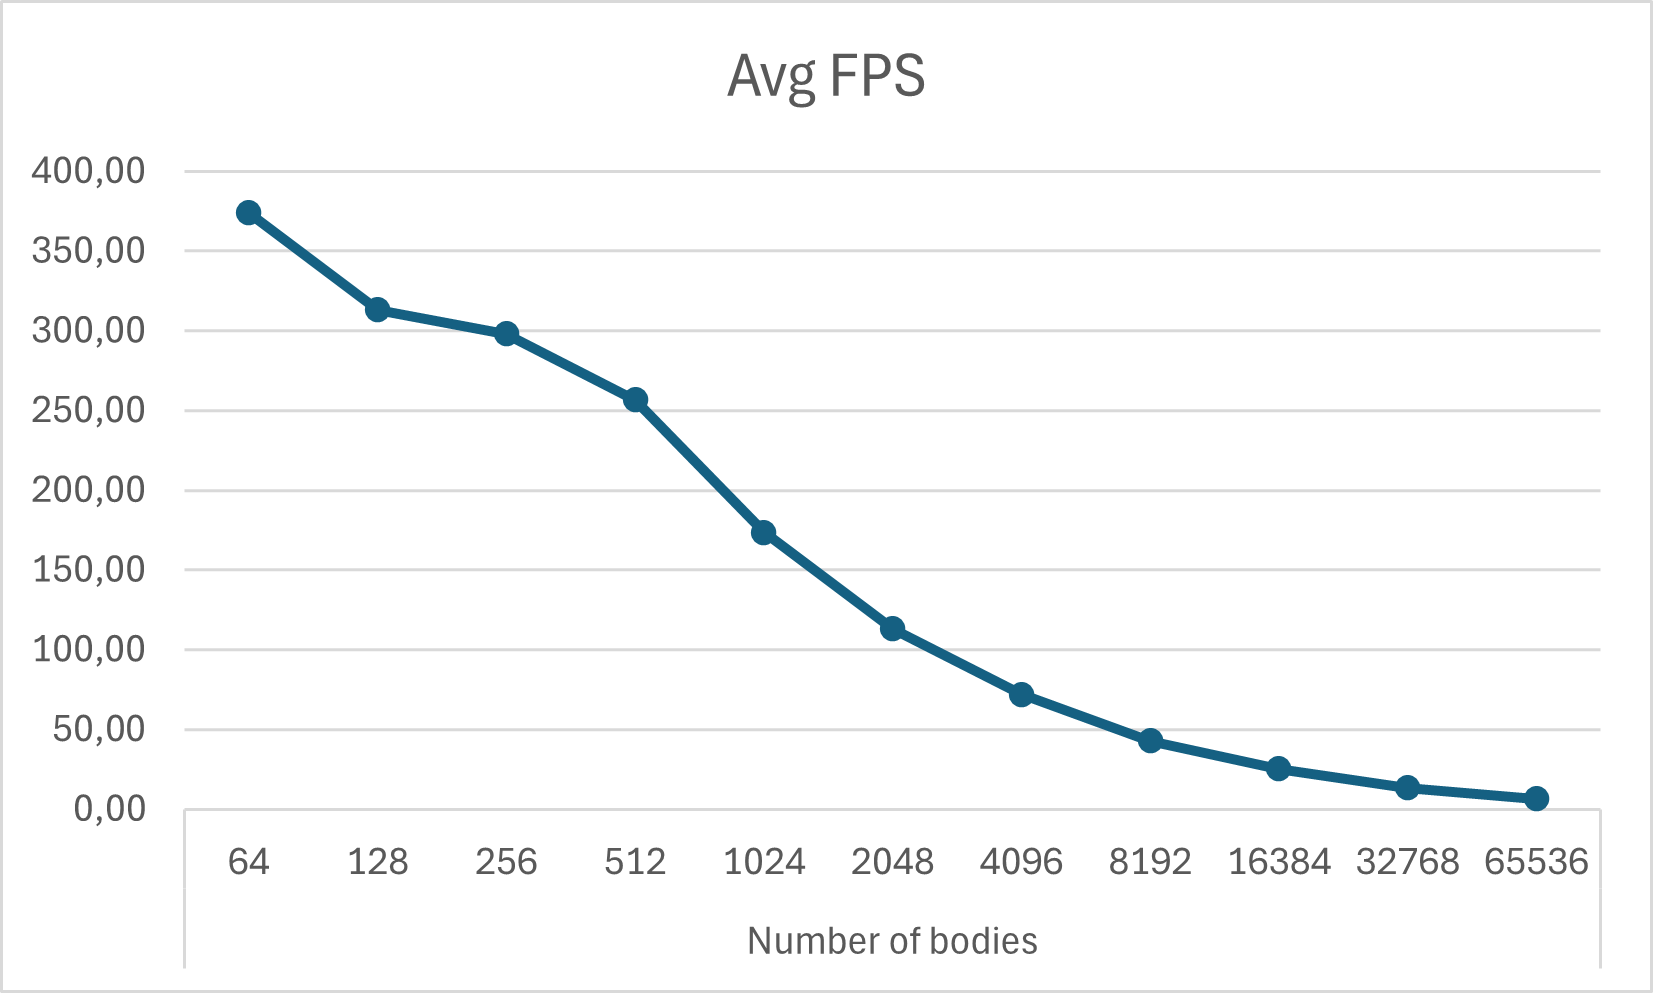
\includegraphics[width=\textwidth]{avgfps.png}
\caption{Average FPS as a function of the number of simulated bodies.
         The curve shows a rapid initial drop at small $N$ followed by
         a smooth super-linear decline consistent with $O(N \log N)$ scaling.}
    \label{fig:fps}
    \end{figure}

    \subsection{Analysis}

    \subsubsection{Two Distinct Regimes}

    The data reveals two clearly distinct performance regimes, visible in
    Figure~\ref{fig:fps}:

\paragraph{Small N (64 -- 512): fixed overhead dominated}

In this range FPS drops from 373 to 257 --- a reduction of only $1.45\times$
despite the body count increasing $8\times$. This indicates that per-frame
work is dominated by \textbf{fixed overhead} that is independent of $N$:

\begin{itemize}
    \item Tree buffer resets (\texttt{enqueueFillBuffer} over the full
          $2N$-node array)
    \item GPU kernel launch latency (7 kernels per frame)
    \item Single-threaded summarize and sort kernels traversing the
          full node array
    \item \texttt{queue.finish()} synchronization cost
\end{itemize}

A linear fit of frame time against $N \log_2 N$ for the full range
yields an estimated fixed overhead of approximately $\mathbf{6.6}$\,ms
per frame, regardless of body count. At $N = 64$, this overhead accounts
for the majority of the 2.67\,ms total frame time.

\paragraph{Large N (1024 -- 65536): $O(N \log N)$ dominated}

Above 1024 bodies the force kernel work becomes dominant and the
$O(N \log N)$ scaling of the Barnes-Hut algorithm becomes clearly visible.
The frame time fits closely to:

\[
t_{\text{frame}} \approx 1.39 \times 10^{-4} \cdot N \log_2 N + 6.6 \;\text{ms}
\]

with residuals under 9\% for all $N \geq 4096$. The table below shows
the measured frame-time doubling ratio when $N$ doubles, alongside the
theoretical prediction:

\begin{table}[h]
\centering
\begin{tabular}{|r|r|r|r|}
\hline
\textbf{N} & \textbf{2N} & \textbf{Measured ratio} & \textbf{$O(N \log N)$ prediction} \\
\hline
4096  & 8192  & 1.68 & 1.92 \\
8192  & 16384 & 1.70 & 1.94 \\
16384 & 32768 & 1.88 & 1.96 \\
32768 & 65536 & 2.03 & 1.97 \\
\hline
\end{tabular}
\caption{Frame-time doubling ratios when $N$ is doubled. The measured ratio
         converges toward the theoretical $O(N \log N)$ prediction as $N$
         grows and fixed overhead becomes negligible.}
\end{table}

As $N$ grows large, the fixed overhead term becomes negligible and the ratio
approaches the theoretical $O(N \log N)$ value. At $N = 65536$ the measured
ratio of 2.03 is within 3\% of the predicted 1.97, confirming that the
force kernel dominates and scales as expected.

\subsubsection{Hardware Observations}

The measurements were taken on an integrated AMD Radeon gfx90c with
7 compute units sharing memory bandwidth with the CPU. Several hardware
constraints affect the absolute numbers:

\begin{itemize}
    \item \textbf{Memory bandwidth:} LPDDR4 shared with the CPU at 42 GB/s.
          At $N = 65536$, each force kernel traversal reads approximately
          $N \cdot \log_2 N \approx 1\,\text{M}$ memory accesses per frame,
          stressing the bandwidth limit.
    \item \textbf{Compute units:} Only 7 CUs are available. The build-tree
          kernel is intentionally limited to \texttt{safe = THREADS = 64}
          total threads to prevent GPU Timeout Detection and Recovery (TDR)
          errors caused by atomic contention on shared tree nodes when too
          many threads compete simultaneously.
    \item \textbf{Thermal throttling:} As an integrated GPU with no dedicated
          cooling, sustained workloads at $N = 65536$ may reduce clock speeds,
          contributing to the slight super-linear increase in frame time
          observed at the high end.
\end{itemize}

\subsubsection{Real-Time Threshold}

A simulation is generally considered interactive if it runs at 30 FPS or above.
Based on the measurements:

\begin{itemize}
    \item Up to $\mathbf{N \approx 8000}$ bodies runs at 30+ FPS on this hardware
    \item $N = 8192$ achieves 42.8 FPS, comfortably above the threshold
    \item $N = 16384$ achieves 25.2 FPS, below 30 FPS but still visually smooth
    \item $N = 65536$ achieves 6.6 FPS, suitable for demonstration but not
          interactive in real time
\end{itemize}

On a discrete GPU with more compute units and dedicated memory bandwidth,
the real-time threshold would shift significantly. The $O(N \log N)$ scaling
means that a GPU with $10\times$ the compute throughput would push the
real-time limit to approximately $N \approx 70000$ bodies.

\subsection{Summary}

The performance measurements confirm that the Barnes-Hut implementation
achieves its expected $O(N \log N)$ time complexity for large particle
counts. The fixed overhead of approximately 6.6\,ms per frame, which includes
kernel launches, buffer resets, and synchronization, limits performance for
small simulations but becomes negligible as $N$ grows.

The simulation maintains real-time performance (above 30 FPS) for up to
approximately 8000 bodies on the tested AMD integrated GPU, and continues
to run at visually useful frame rates up to 65536 bodies.

\end{document}